\chapter{The Social AR Continuum} % Main chapter title
\label{ch:continuum} % Change X to a consecutive number; for referencing this chapter elsewhere, use \ref{ChapterX}

This chapter describes The Social AR Continuum, a space that encompasses different dimensions of Augmented Reality (AR) for sharing social experiences. We explore various dimensions, discuss options for each dimension, and outline possible scenarios where these options might be useful. We categorise the social AR dimensions into three areas: 1) Self and others or people, 2) Surrounding environment and objects, and 3) Interactions.

Representing self and others as avatars is described in more detail in Chapter \ref{ch:contacts}. The surrounding environment and sharing different types of data is described in more detail in Chapter \ref{ch:data}, while the interactions between people in the form of annotation on the surrounding environment are described in Chapter \ref{ch:annotation}.

% \section{Concept}
% \section{General System Implementation}
% \section{Evaluation}

% =============== PREVIOUS WORK ================
% A. Nassani, G. Lee, M. Billinghurst, T. Langlotz, S. Hoermann and R. W. Lindeman, “[Poster] The Social AR Continuum: Concept and User Study” in ISMAR 2017
% =============== PREVIOUS WORK ================

% \section{Abstract}
% \label{sec:continuum-abstract}

In this work, we describe The Social AR Continuum, a space that encompasses different dimensions of Augmented Reality (AR) for sharing social experiences. We explore various dimensions, discuss options for each dimension, and explore possible scenarios where these options might be useful. 

\begin{figure}
    \centering
    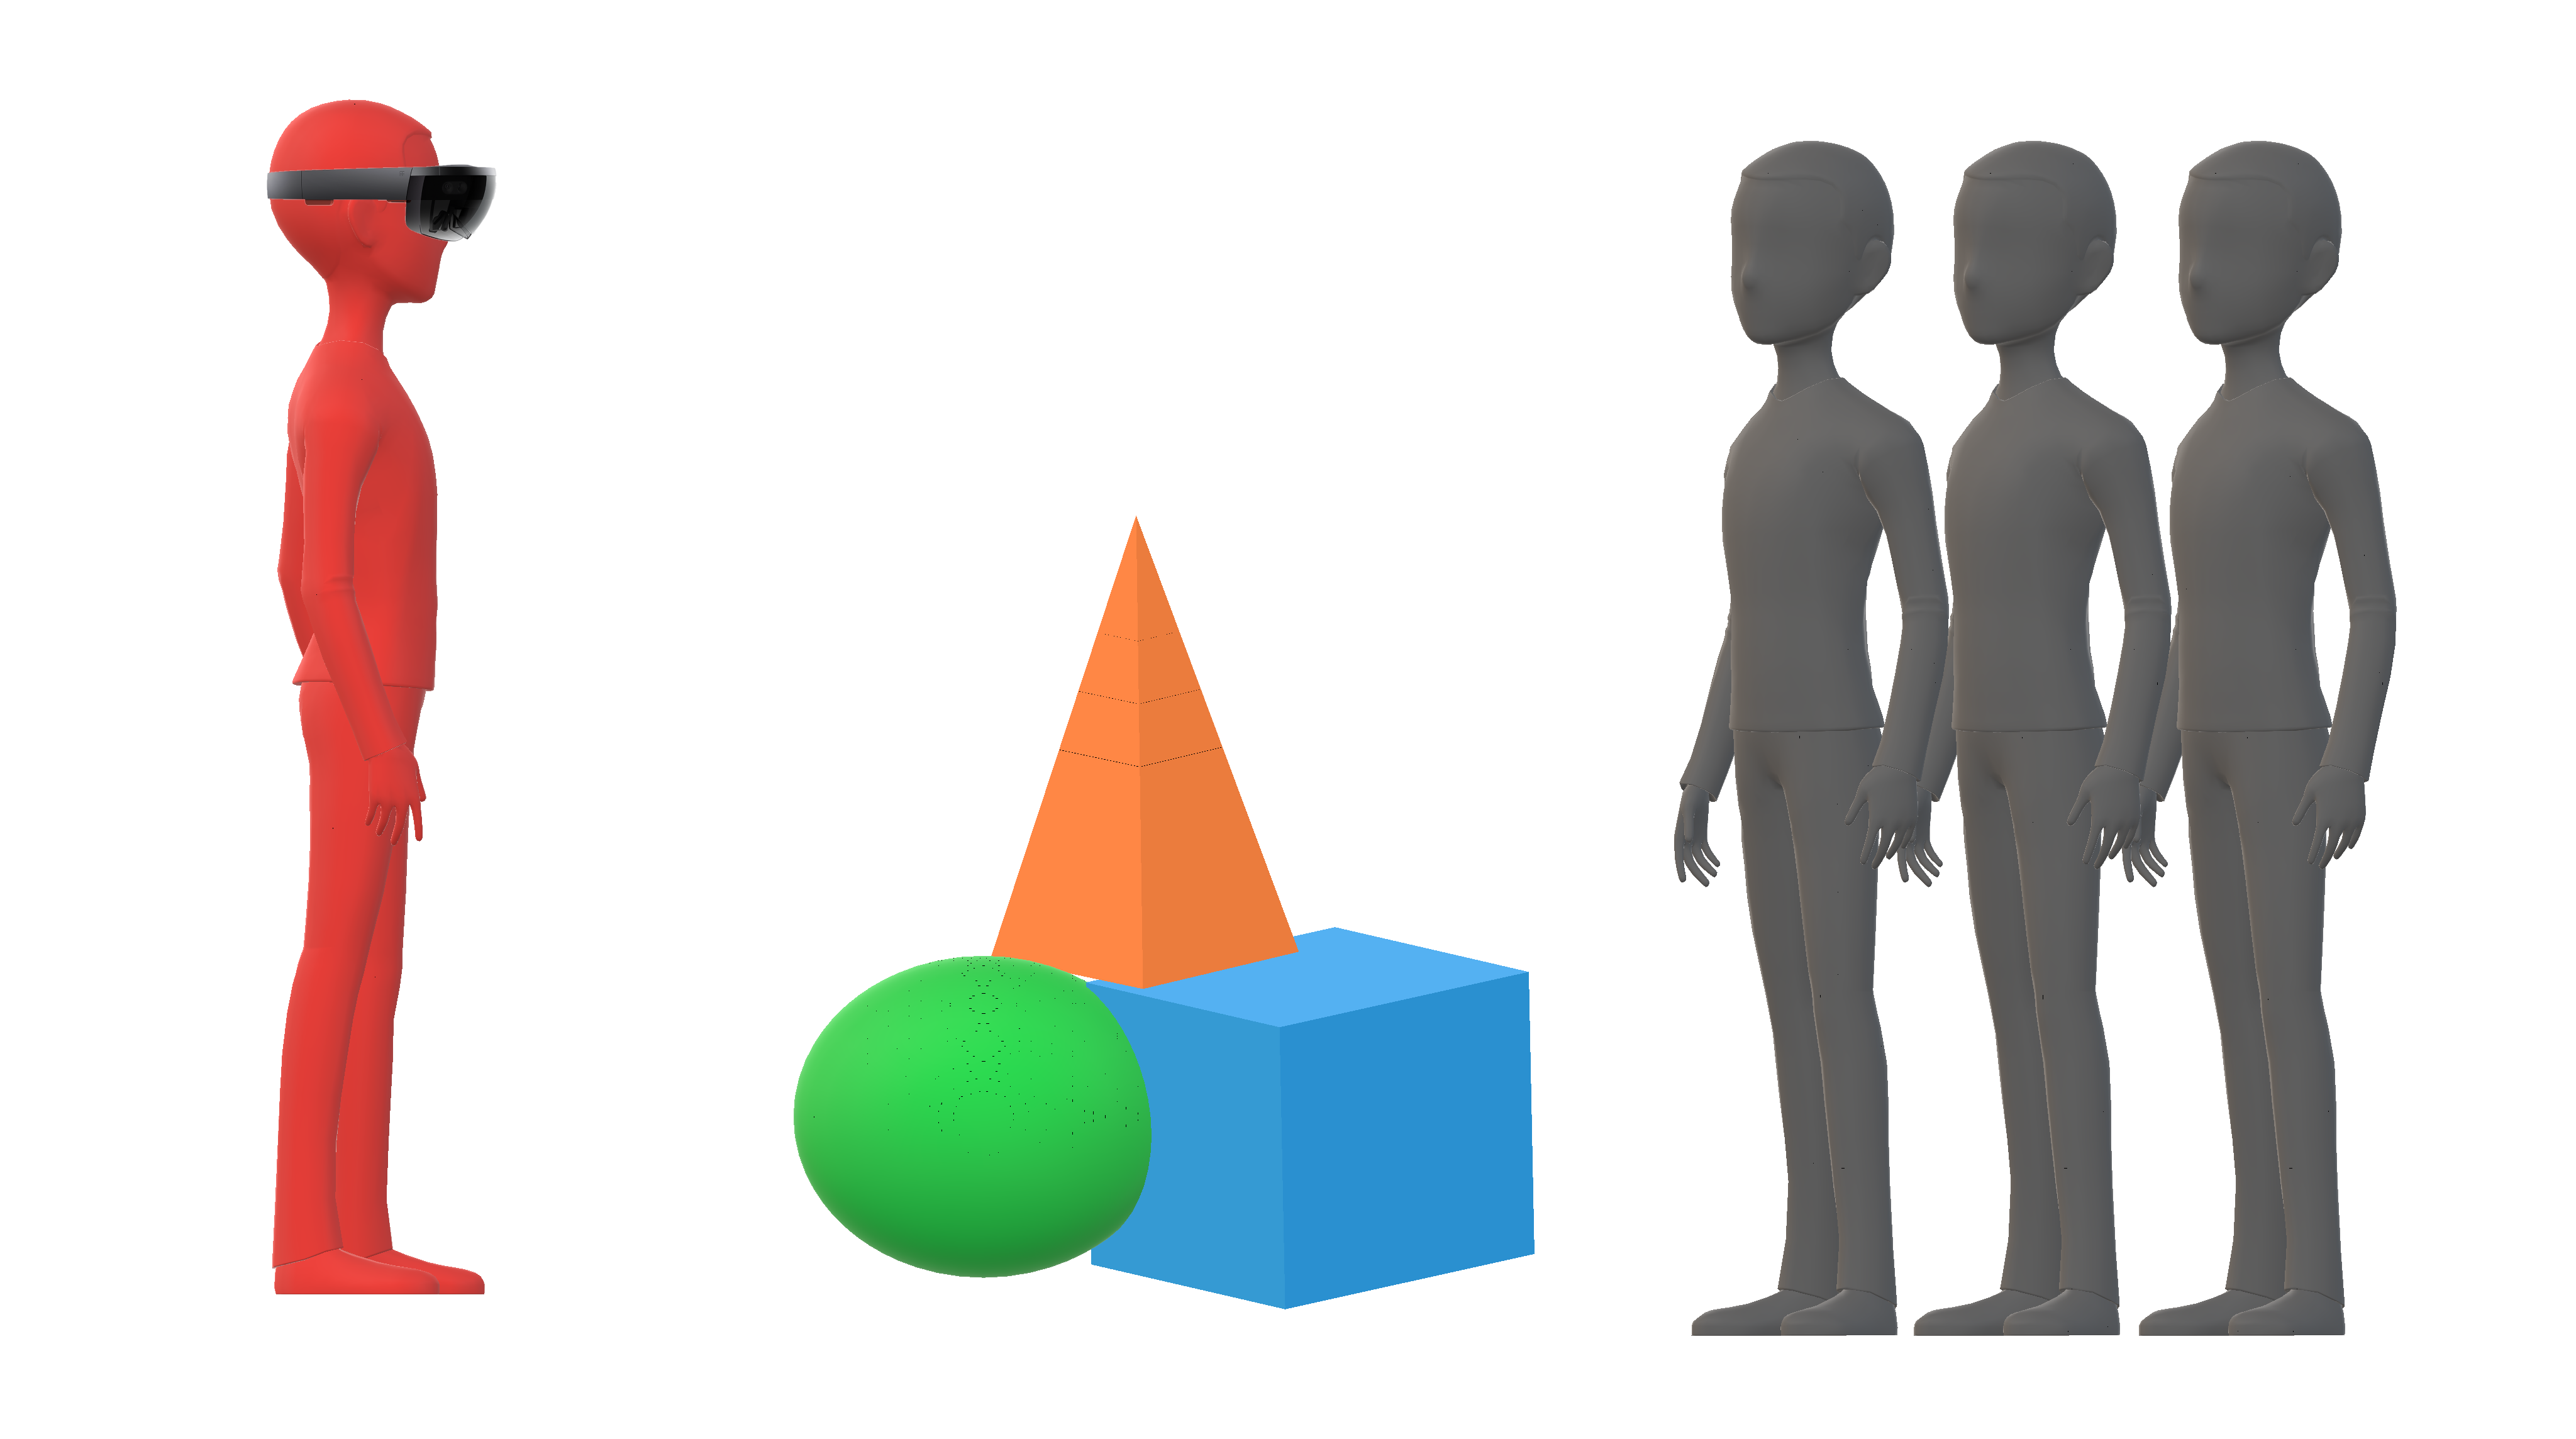
\includegraphics[width=3in]{images/continuum_categories5.png}
    \caption{The social AR continuum categories: 1) self and others, 2) objects and surrounding environments, 3) interaction and annotations}
    \label{fig:continuum:categories}
\end{figure}


This work aims to layout the space of the AR continuum for social sharing experiences by looking at parameters and options that can be changed in terms of people, objects and the environment to create a shared AR experience.

\section{Social AR Continuum Dimensions}

As we established the social AR continuum varies based on the closeness of social connections that we have with others (relationship), we identified the following dimensions where social AR applications can fit along a continuum. The dimensions can be grouped in the categories described in Figure \ref{fig:continuum:dimensions}.

\begin{figure}
    \centering
    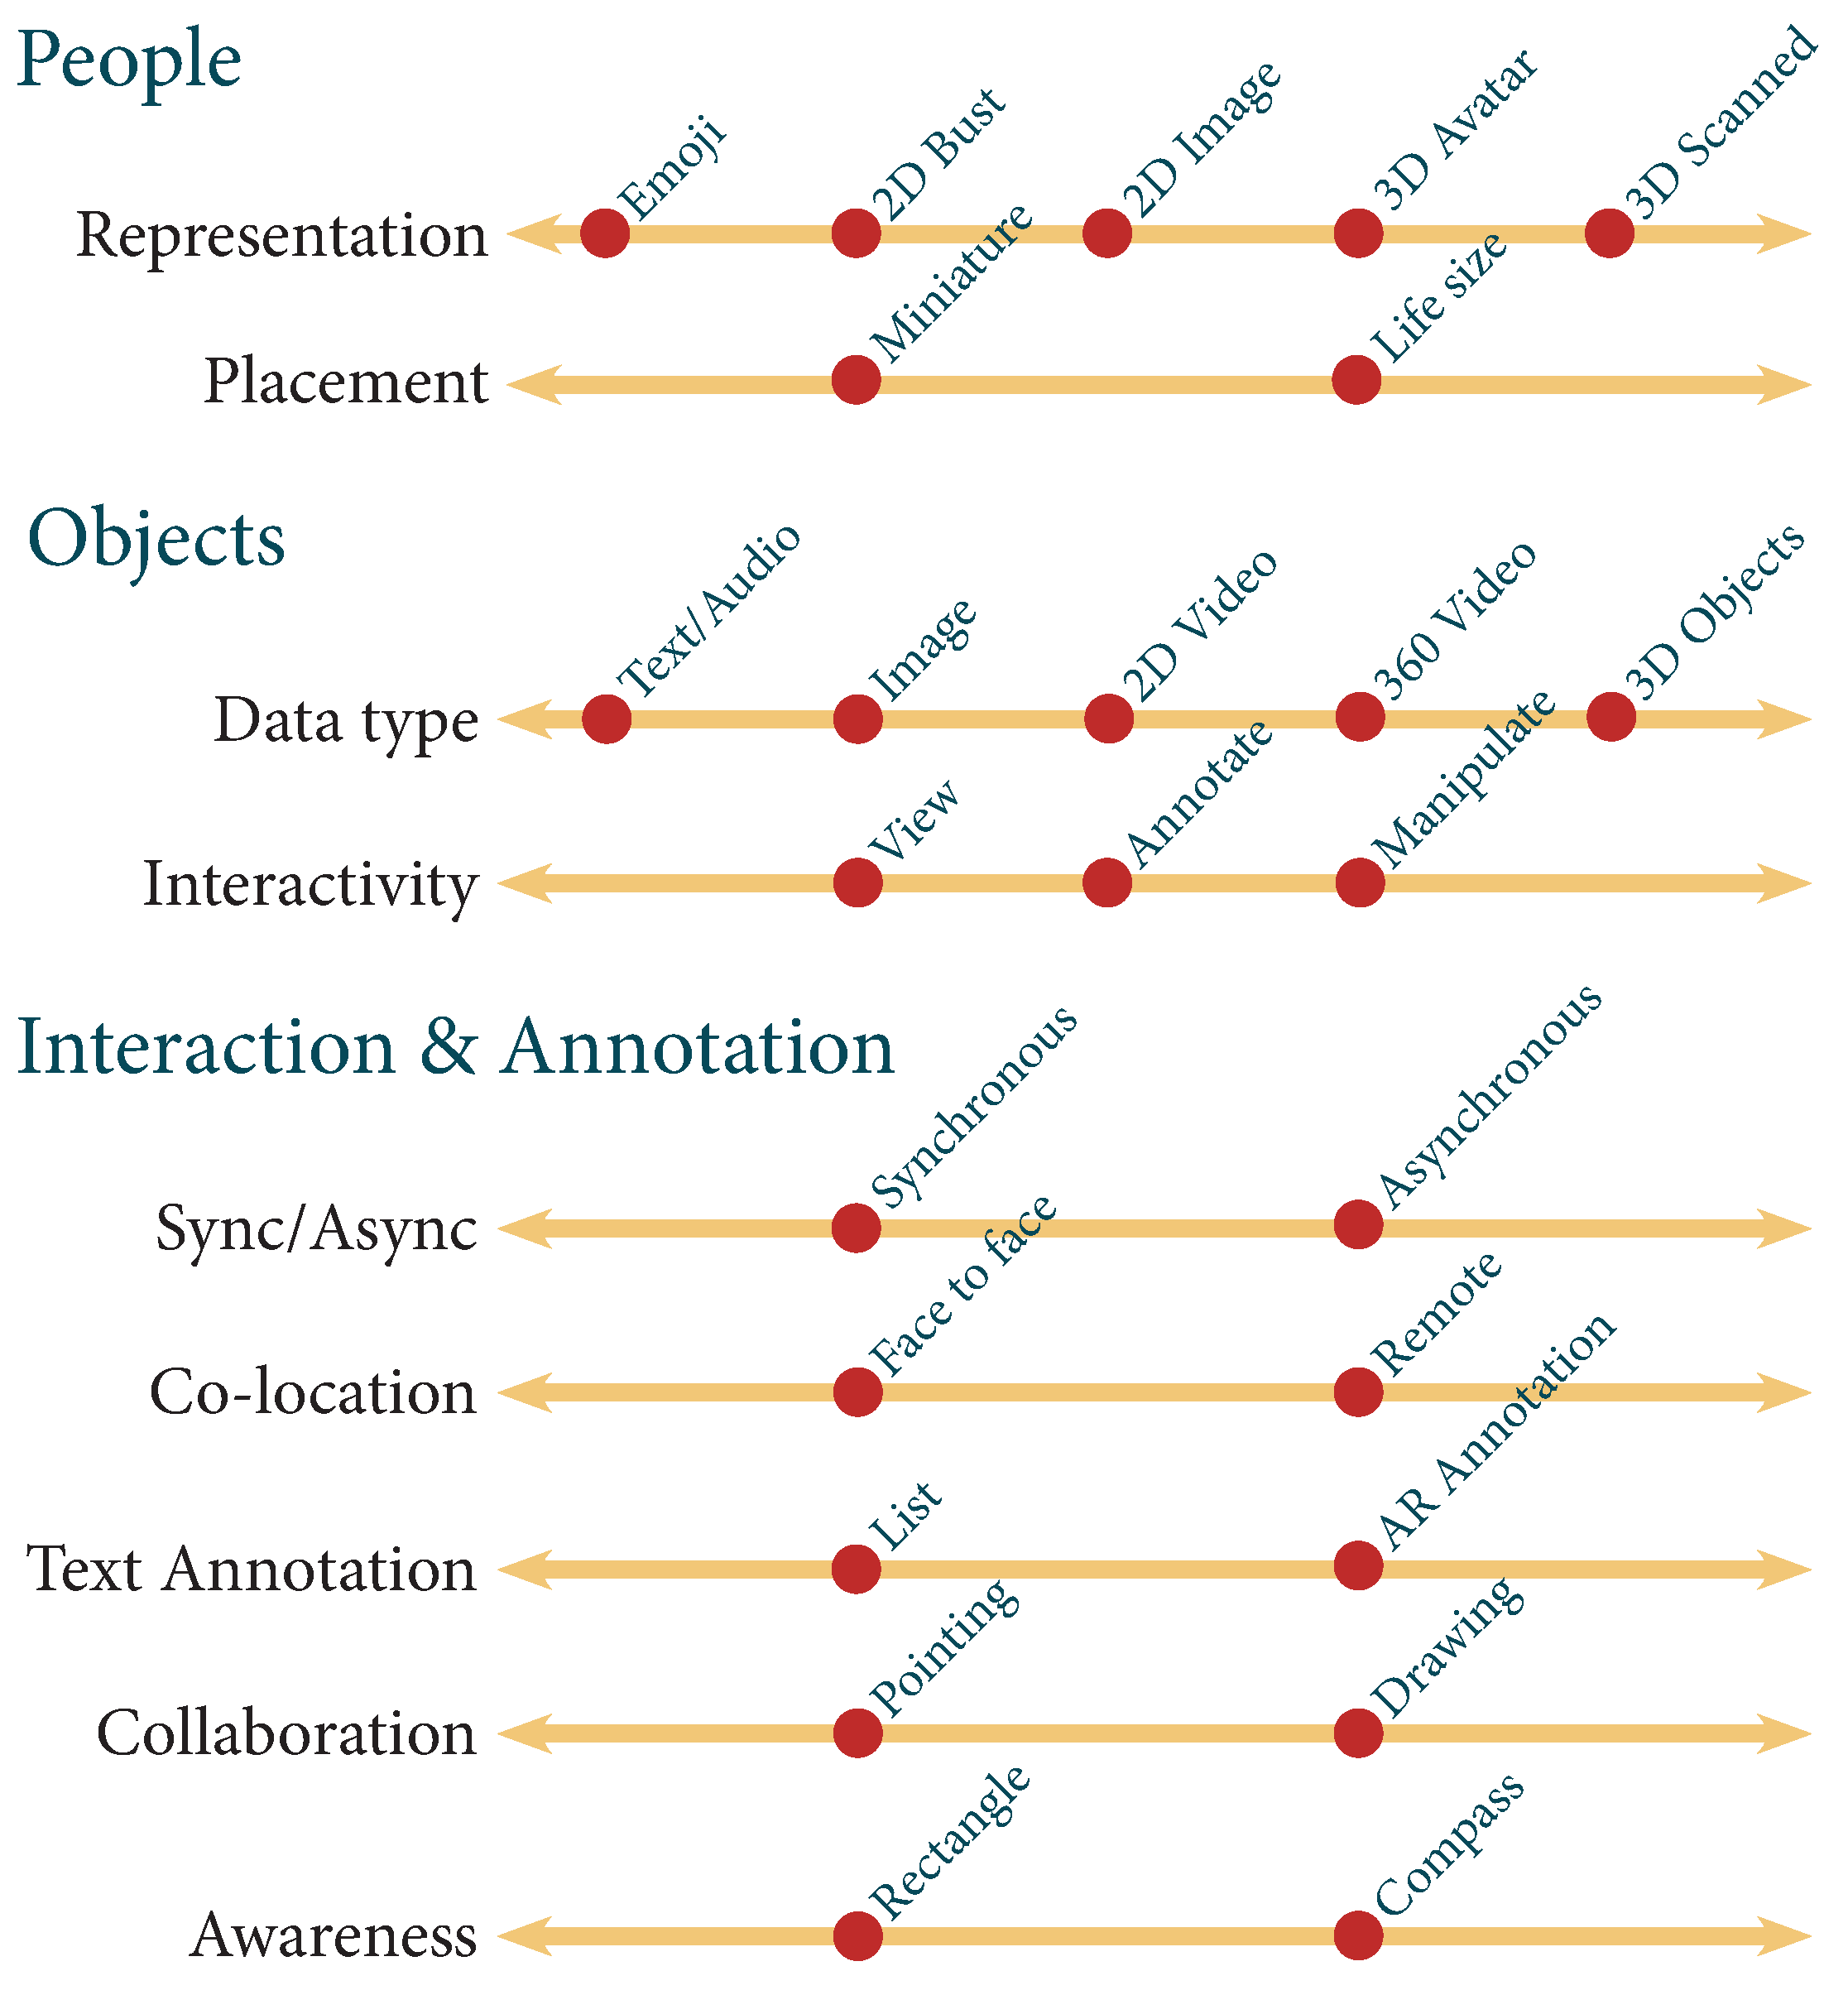
\includegraphics[width=.8\linewidth]{images/continuum4.1.eps}
    \caption{Dimensions of Social AR Continuum}
    \label{fig:continuum:dimensions}
\end{figure}

\textbf{Contact Representation}

Representing social contacts can vary on the social AR continuum based on the relationship that the user has with the contact. Intimate contacts can be represented as full 3D animated avatars. Friends could be represented as 2D static images, while Acquaintances could be represented as 2D busts and strangers as mere emojis. Each contact could choose their representation for each category.  

\begin{figure}[h]
    \centering
    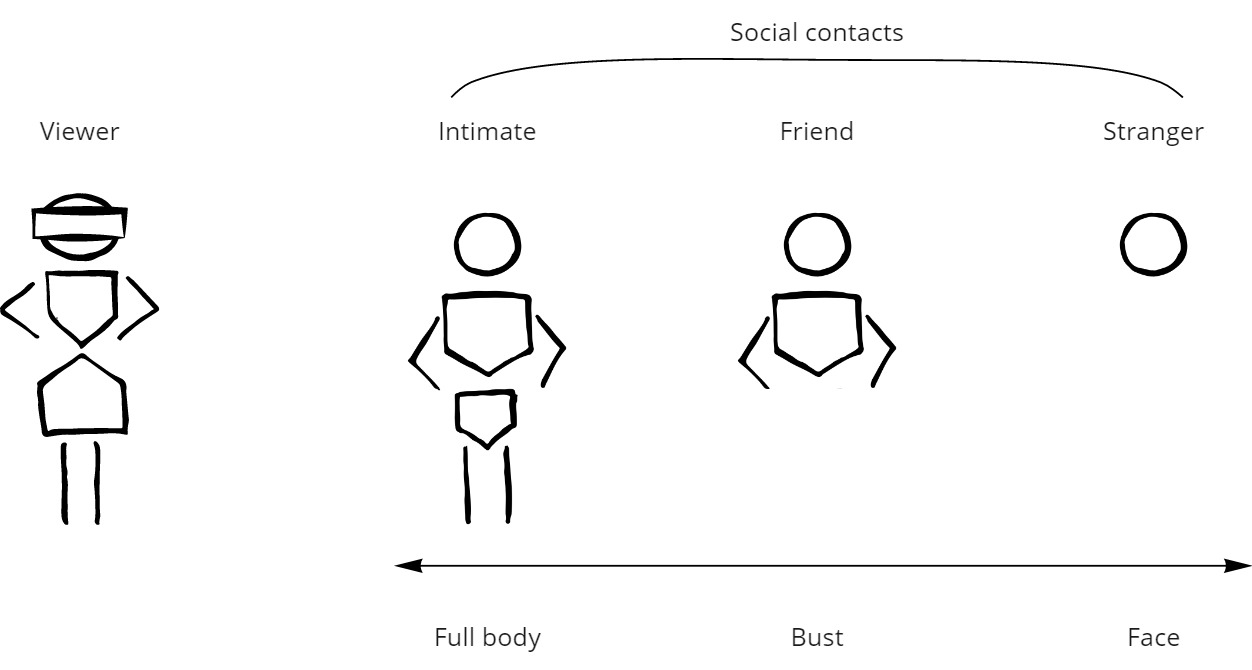
\includegraphics[width=.8\linewidth]{images/Continuum-representation.jpg}
    \caption{Contact representation}
    \label{fig:continuum:contact-representations}
\end{figure}

% \textbf{Contact Filter}
% Filtering social contacts to distinguish users from each other could be done using proximity or visual fidelity based on their relationship to the user. Proximity filters contacts by placing them closer or further away. Visual fidelity filters contacts by adding more level of detail to the contact for closer relationships and less detail for further away contacts. 

\textbf{Contact Placement}
Placing social contacts can be done either by displaying them as life-size avatars on the ground around the user for close relationships or by displaying them as miniatures on a distant surface. 

\begin{figure}[h]
    \centering
    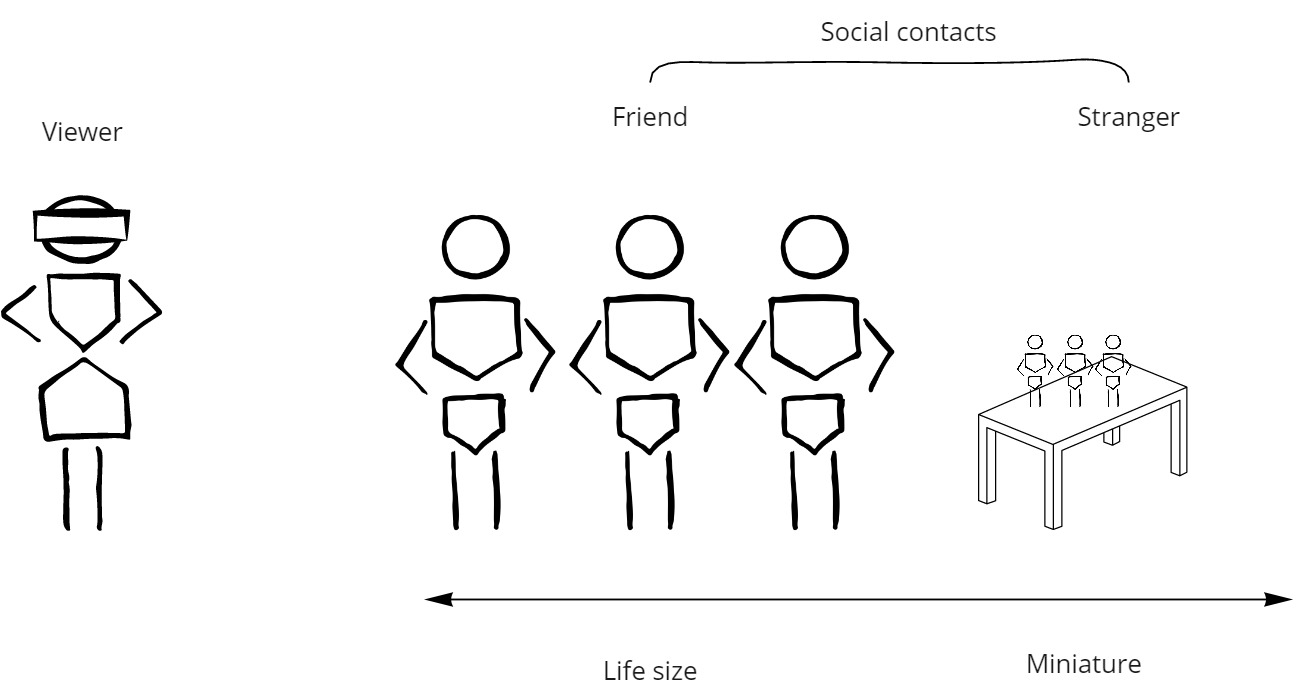
\includegraphics[width=.8\linewidth]{images/Continuum-placement.jpg}
    \caption{Contact placement}
    \label{fig:continuum:contact-placement}
\end{figure}

\textbf{Data Type}
The type of data shared between social contacts in AR can be categorised as 1D (e.g., text or audio), 2D (e.g., images, panorama or video), or 3D (e.g., 3D model or scanned-room environment). Based on the relationship between the user and his/her social contacts, the type of data available can be filtered. For instance, 3D data are shared with intimate relationships, while acquaintances can see only 2D data.  

\begin{figure}[h]
    \centering
    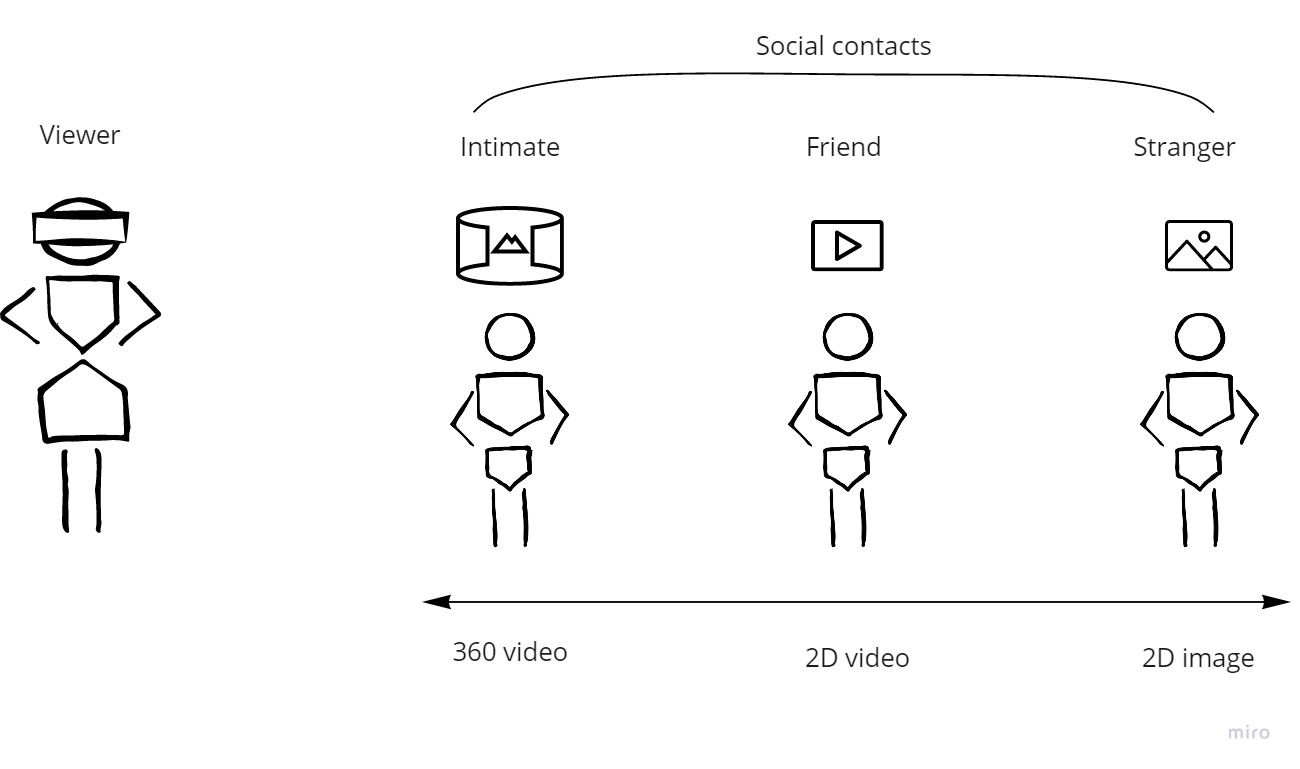
\includegraphics[width=.8\linewidth]{images/Continuum-Data-type.jpg}
    \caption{Data type}
    \label{fig:continuum:data-type}
\end{figure}

\textbf{Data interactivity}
In terms of user interactions with shared data, the continuum here ranges from viewing the contents, annotating or adding comments on the content, through to manipulating the content. Levels of manipulation include changing the position, rotation or scale of the shared content, or even modifying the content itself.

\begin{figure}[h]
    \centering
    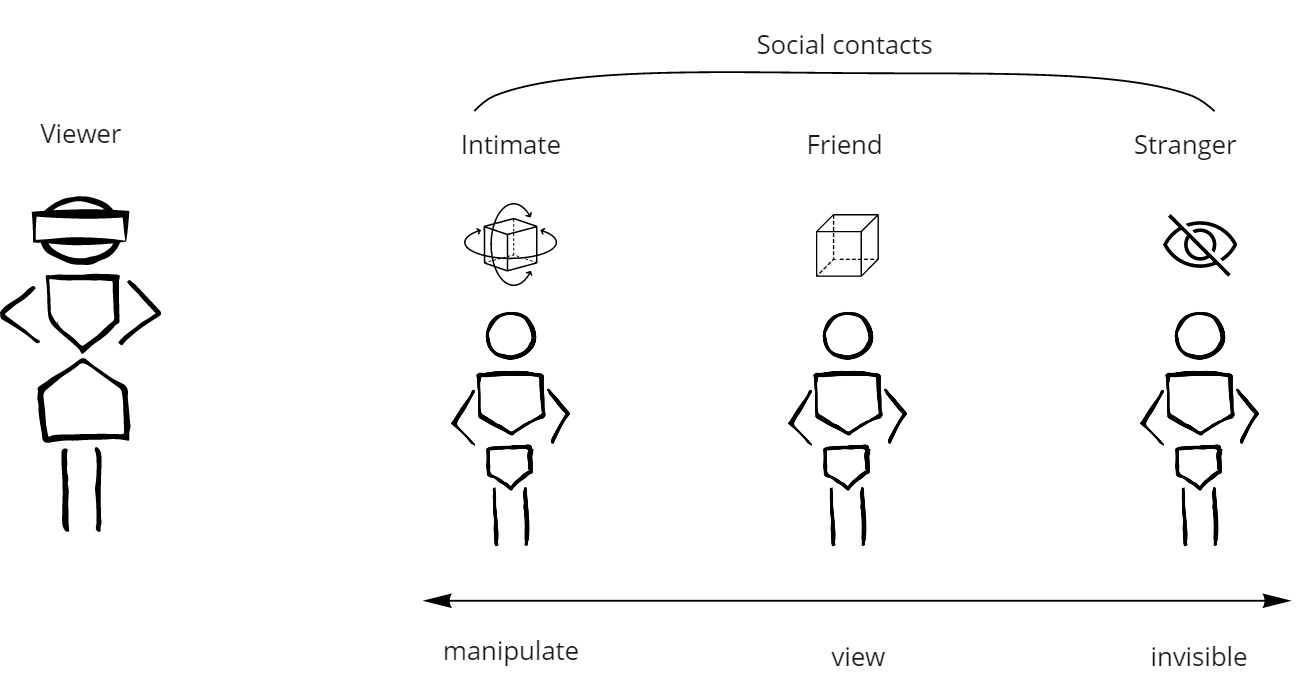
\includegraphics[width=.8\linewidth]{images/Continuum-interaction.jpg}
    \caption{Data interactivity}
    \label{fig:continuum:data-interaction}
\end{figure}

% \textbf{Data Privacy}
% Based on the relationship with other users, shared data can be made private to the user, shared with specific groups of people (e.g., friends, acquaintances), or shared with everyone. 

\textbf{Sync/Async}
The data shared with contact can be shared in a synchronous way where both sharing and interaction happen at the same time. In contrast, data can also be shared asynchronously \cite{Smith2016}, i.e., interaction happens at a different time. 

\begin{figure}[h]
    \centering
    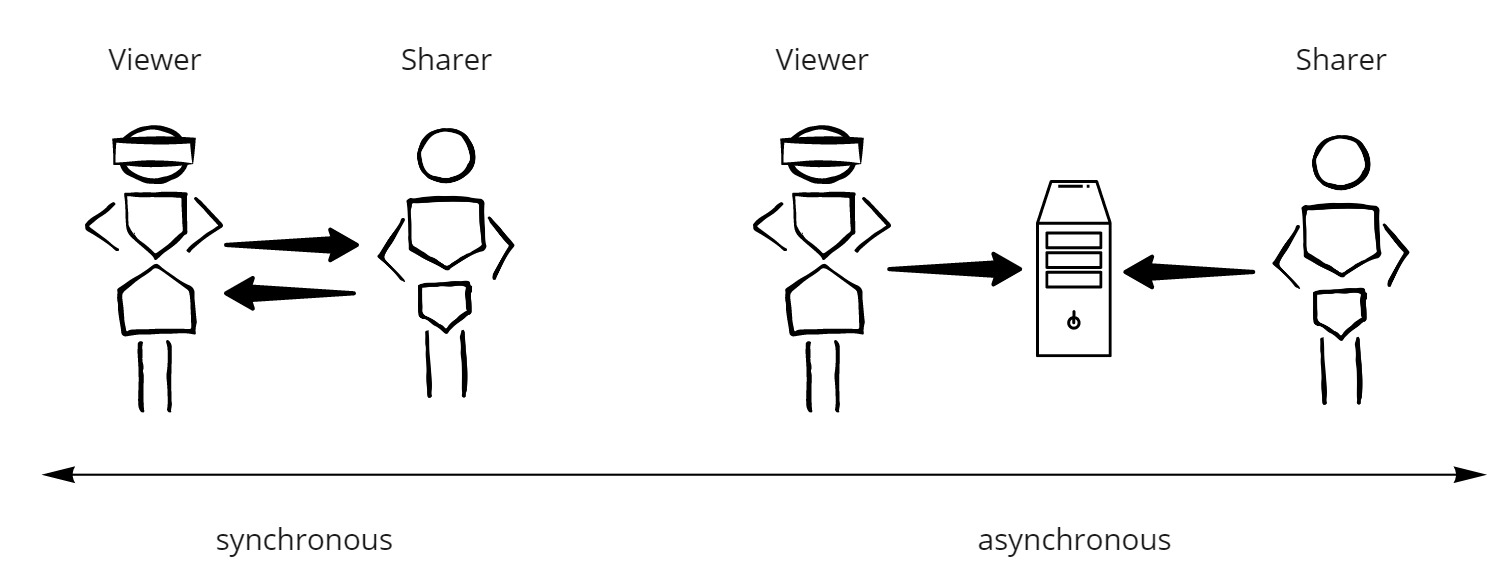
\includegraphics[width=.8\linewidth]{images/continuum-connection.jpg}
    \caption{Data connection}
    \label{fig:continuum:data-connection}
\end{figure}

\textbf{Co-location}
Social contacts can either be remote (i.e., in a different place than the user) or face-to-face (i.e., physically in the same location as the user). When social contacts are remote, they are represented as virtual avatars based on their relationship with the user. An example of face-to-face interaction was described in a Black Mirror \footnote{http://www.imdb.com/title/tt2085059/} episode where a person could 'block' another co-located person by blurring them out in their AR view of the real world.

\begin{figure}[h]
    \centering
    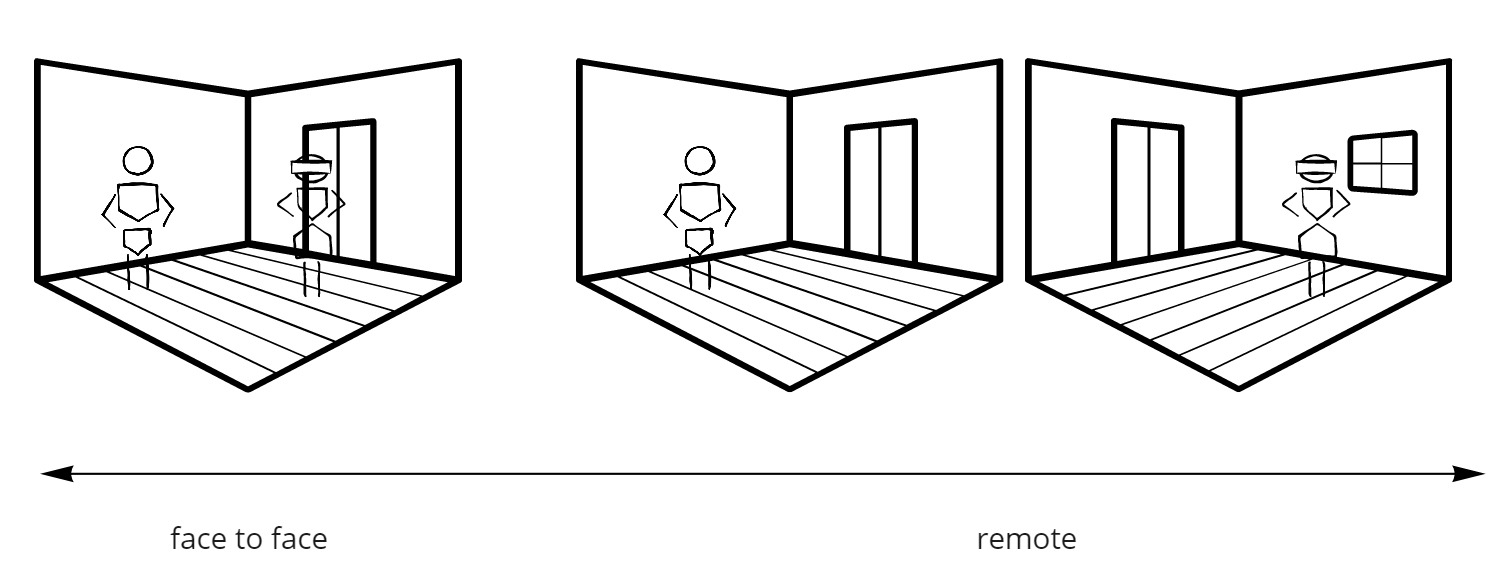
\includegraphics[width=.8\linewidth]{images/continuum-colocation.jpg}
    \caption{Data colocation}
    \label{fig:continuum:data-colocation}
\end{figure}


\textbf{Text Annotation}
When adding text to describe an object or a place, the text can be placed as a list (lower fidelity) on the side of the screen or can be placed on the related object as an AR annotation (higher fidelity) that sticks with the scene and disappears if the user looks away. This dimension can be used with social contacts that if the contact is a close friend then would see the annotation in higher fidelity, and in case of a stranger, the text annotation becomes less fidelity. 

\textbf{Collaboration}
When collaborating with social contacts, the user could use a pointer (e.g. arrow, indicator) to direct the conversation to a particular place or use drawing tool (e.g. pencil) to highlight the area of the conversation. The availability of these options could depend on the social proximity between social contacts. If closer to each other, higher fidelity tools are available, and if strangers then the collaboration is limited to lower fidelity tools.

\textbf{Awareness}
It is possible during a session of sharing social experiences, that social contacts are looking in different directions awareness tools help users to know where the other user is looking at. This can be achieved by showing a rectangle or a circle pointing to where the user is looking, or by using a context compass view which provides higher fidelity for closer connections.

\section{Summary}

In this work, we introduced the concept of The Social AR Continuum. We identified several dimensions where a social AR application could be implemented.
